\documentclass[fontsize=12pt]{scrartcl}

\newcommand{\grad}{\ensuremath{^{\circ}} }
\renewcommand{\strut}{\vrule width 0pt height5mm depth2mm}

\usepackage[utf8]{inputenc}
\usepackage[final]{pdfpages}
% obere Seitenränder gestalten können
\usepackage{fancyhdr}
\usepackage{moreverb}
% Graphiken als jpg, png etc. einbinden können
\usepackage{graphicx}
%\usepackage{stmaryrd}
% Floats Objekte mit [H] festsetzen
\usepackage{float}
% setzt URLs schön mit \url{http://bla.laber.com/~mypage}
\usepackage{url}
% Externe PDF's einbinden können
\usepackage{pdflscape}
% Verweise innerhalb des Dokuments schick mit " ... auf Seite ... "
% automatisch versehen. Dazu \vref{labelname} benutzen
\usepackage[ngerman]{varioref}
\usepackage[ngerman]{babel}
\usepackage{ngerman}
% Bibliographie
\usepackage{bibgerm}
% Tabellen
\usepackage{tabularx}
\usepackage{supertabular}
\usepackage[colorlinks=true, pdfstartview=FitV, linkcolor=blue,
            citecolor=blue, urlcolor=blue, hyperfigures=true,
            pdftex=true]{hyperref}
\usepackage{bookmark}
\usepackage[a4paper, twoside]{geometry}

% Damit Latex nicht zu lange Zeilen produziert:
\sloppy
%Uneinheitlicher unterer Seitenrand:
%\raggedbottom

% Kein Erstzeileneinzug beim Absatzanfang
% Sieht aber nur gut aus, wenn man zwischen Absätzen viel Platz einbaut
\setlength{\parindent}{0ex}

% Abstand zwischen zwei Absätzen
\setlength{\parskip}{1ex}

\addtolength{\evensidemargin}{-2cm}
\addtolength{\oddsidemargin}{2cm}

% Lustige Header auf den Seiten
  \pagestyle{fancy}
  \setlength{\headheight}{70.55003pt}
  \fancyhead{}
  \fancyhead[LO,RE]{Benutzerhandbuch}
  \fancyhead[LE,RO]{Seite \thepage\\\slshape \leftmark\\\slshape \rightmark}

%
% Und jetzt geht das Dokument los....
%

\begin{document}

% Start Titelseite
  \thispagestyle{empty}
  \newgeometry{hmarginratio=1:1}
  \vspace{3cm}
  \begin{minipage}[H]{\textwidth}
  \begin{center}
  \vspace{1cm}
  \bf
  {\Large Benutzerhandbuch}\\
  der Stundenplansoftware \\
  der Gruppe\\
    \begin{figure}[H]
    \centering
    
\includegraphics[width=0.15\textwidth]{../WOYM.png}
    \end{figure}
  \vfill
  \end{center}
  \end{minipage}
  \vfill
  \begin{minipage}[H]{\textwidth}
  \begin{center}
  \sf
  \begin{tabular}{l}
  Tim Hansen \\
  Joshua Hoffmann\\
  Hassan Klait \\
  Adrian Lück \\
  Jurij Schmidt\\
  Falko Schröder
  \end{tabular}
  \end{center}
  \end{minipage}
\restoregeometry
% Ende Titelseit

% Start Leerseite
\cleardoubleemptypage

%Start Inhaltsverzeichnis
\newpage

  \thispagestyle{fancy}
  \fancyhead{}
  \fancyhead[LO,RE]{Benutzerhandbuch\\ \mbox{}\\}
  \fancyhead[LE,RO]{Seite \thepage\\\slshape \leftmark\\~}
  \fancyfoot{}
  \renewcommand{\headrulewidth}{0.4pt}
  \tableofcontents

\newpage

  \fancyhead[LE,RO]{Seite \thepage\\\slshape \leftmark \\\slshape \rightmark}

\section{Einleitung}
Sehr geehrter Nutzer, sehr geehrte Nutzerin,\\
vielen Dank, dass sich für unsere Stundenplansoftware entschieden haben. Auf den folgenden Seiten sollen Sie Schritt für Schritt, über die Installation bis hin zum Erstellen und Anzeigen von Stundenplänen, an die Software herangeführt werden. 

\clearpage 

\section{Installation und Inbetriebnahme}
\subsection{Installation und Inbetriebnahme auf Windows Systemen}
\subsection{Installation und Inbetriebnahme auf Linux/Mac OS Systemen}

\clearpage

\section{Bedienung der Software}

\subsection{Die Einrichtungsseite}
Die Einrichtungsseite dient der Vorbereitung zur Planung. Sie legen dort Standorte und Räume, Unterrichtsinhalte, Schulklassen und Personen des Personals an. Es wird empfohlen im Navigationsmenü auf der linken Seite von oben nach unten vorzugehen.

\subsubsection{Hinzufügen eines Objektes am Beispiel einer Lehrkraft}
\begin{enumerate}
\item Klicken Sie im Menü auf der linken Seite auf den Eintrag "`Lehrkräfte"'.
\item Sie sehen nun eine Tabelle, in welcher alle vorhandenen Lehrkräfte angezeigt werden. Klicken Sie auf den "`Hinzufügen"'-Button oben rechts.
\item Das folgende Dialogfenster öffnet sich: \medskip\\
	\begin{minipage}[t]{\linewidth}
            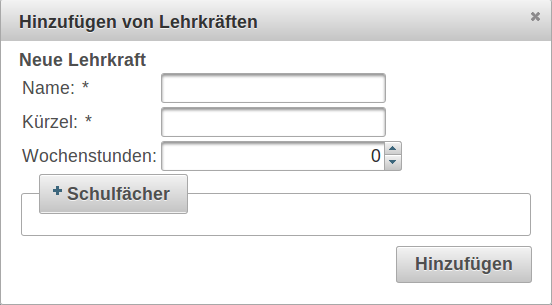
\includegraphics[width=.8\linewidth]{images/addTeacherDialog.png}
    \medskip\\
    Die mit * gekennzeichneten Angaben sind Pflichtangaben. Aufklappbare Angaben sind immer optional.
    \end{minipage}
\clearpage
\item Machen Sie alle gewünschten Angaben und klicken Sie anschließend auf "`Hinzufügen"'. Sie werden darüber informiert, wenn das Hinzufügen erfolgreich war: \medskip\\
	\begin{minipage}[t]{\linewidth}
          %TODO:Aktualisieren
            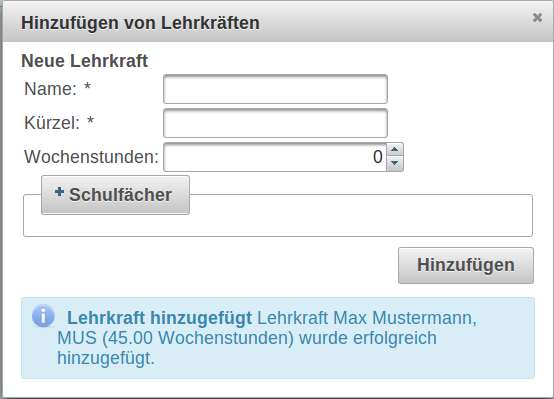
\includegraphics[width=.8\linewidth]{images/addedTeacher.png}
    \medskip\\
    Das Dialogfenster bleibt geöffnet, um das Hinzufügen weiterer Lehrkräfte zu erlauben. Wenn Sie keine weitere Lehrkraft hinzufügen möchten, klicken Sie auf das X in der oberen rechten Ecke des Dialogs.
    \end{minipage}
\end{enumerate}

\subsubsection{Aktualisieren eines Objektes am Beispiel einer Lehrkraft}

\begin{enumerate}
\item Führen Sie einen Rechtsklick auf die zu bearbeitende Lehrkraft aus und wählen sie "`Bearbeiten"': \medskip\\
	\begin{minipage}[t]{\linewidth}
          %TODO:Aktualisieren
            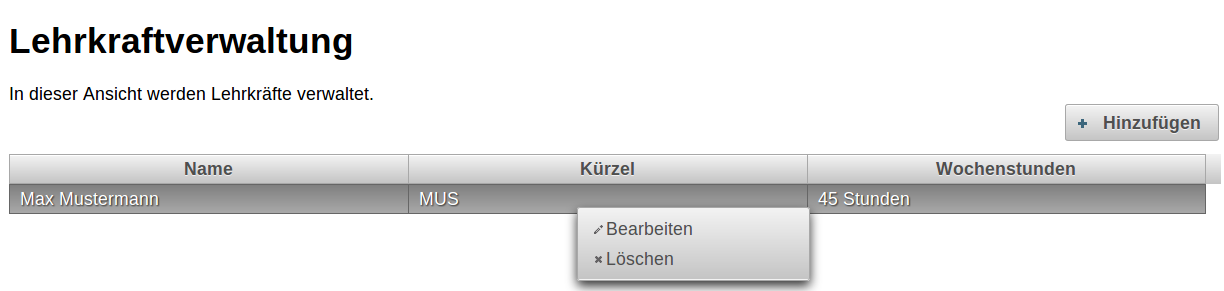
\includegraphics[width=1\linewidth]{images/editTeacher.png}
    \end{minipage}
\item Im dem sich öffnenden Dialogfenster sind alle Angaben der gewählten Lehrkraft eingetragen: \medskip\\
	\begin{minipage}[t]{\linewidth}
          %TODO:Aktualisieren
            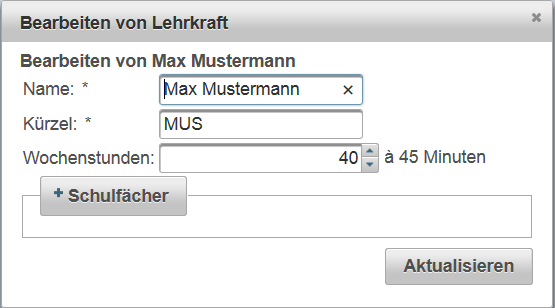
\includegraphics[width=.8\linewidth]{images/editTeacherDialog.png}
    \medskip\\ Passen Sie die Angaben nach Belieben an.
    \end{minipage}
\item Klicken Sie auf "`Aktualisieren"'. Bei Erfolg schließt sich das Dialogfenster und Sie werden über die erfolgreiche Aktualisierung informiert. %TODO: Erweitern
\end{enumerate}



\end{document}
